\section{Maximum Likelihood Estimator (mle)}

We continue the concepts of samples and statistics in chapter 2 while introducing the main tools of inference: confidence intervals and tests of hypotheses.
In a typical statistic problem, we have $X$ but don't know its pdf $f(x)$ or pmf $p(x)$. There are two cases: completely unkown and known down to a parameter $\theta$ which may be a vector. Now we consider the second case, e.g. $X\sim Exp(\theta)$ with unkown $\theta$, $X\sim N(\mu,\sigma^{2})$ with unknown $\mu,\sigma^{2}$.
$X_1,X_2,\dots,X_n$ idd is called a \textbf{random sample} of size $n$, and a function of the sample  $T=T(X_1,\dots,X_n)$  is called a \textbf{statistic}. Once the sample is drawn, then $t$ is called the \textbf{realization} of $T$, where $t=T(x_1,\dots,x_n)$ and $x_1,\dots,x_n$ is the realization of the sample.

\begin{figure}[H]
\centering
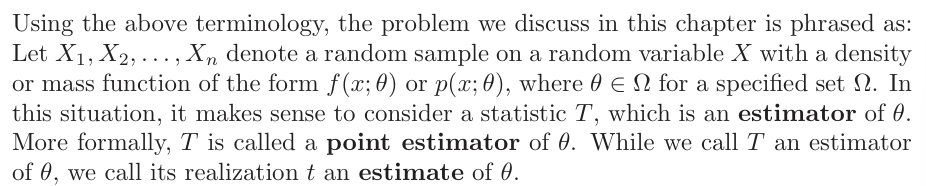
\includegraphics[width=\textwidth]{chap4-20250313.png}
% \caption{}
\label{}
\end{figure}

\begin{figure}[H]
\centering
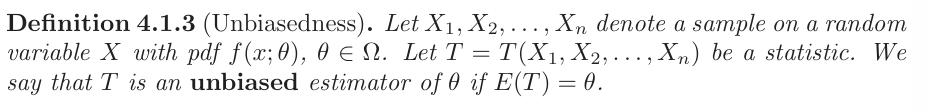
\includegraphics[width=\textwidth]{1-chap4-20250313.png}
% \caption{}
\label{}
\end{figure}

In chapter 6 and 7 we discuss several theories of estimation in general. We briefly discuss the \textbf{maximum likelihood estimator (mle)} and then use it to obtain point estimators. Our discussion is for the continuous case.
The information is involved in the \textbf{likelihood function} $L(\theta)=L(\theta;x_1,\dots,x_n)=\prod_{i=1}^{n}f(x_i;\theta)$. An often-used estimate is the value of $\theta$ that provides a maximum of $L(\theta)$. If unique, this is called the \textbf{maximum likelihood estimator} (mle) and we denote it as $\widehat{\theta}=\mathrm{Argmax}\ L(\theta)$. In practice, it's easier to work with $l(\theta)=\log L(\theta)$, and $\widehat{\theta}$ solves $\frac{ \partial l(\theta) }{ \partial \theta }=0$.

\subsection{Examples}

\subsubsection{Exponential Distribution}

Suppose $X_1,\dots ,X_n\sim\Gamma(1,\theta)$ with density $f(x)=\theta ^{-1}\exp \{ -x/\theta \}$, $0<x<\infty$. The log of the likelihood function is given by
\[
l(\theta)=\log \prod_{i=1}^{n} \frac{1}{\theta} e^{ -x_i/\theta }=-n\log\theta-\theta ^{-1}\sum_{i=1}^{n} x_i
\]
The first partial of the log-likelihood with respect to $\theta$ is
\[
\frac{ \partial l(\theta) }{ \partial \theta } =-n\theta ^{-1}+\theta^{-2}\sum_{i=1}^{n} x_i
\]
Setting this partial to 0 then we obtain the solution $\overline{x}$, thus the statistic $\hat{\theta}=\overline{X}$ is the mle of $\theta$. Because $E(X)=\theta$ we have $E(\overline{X})=\theta$ hence $\hat{\theta}$ is an unbiased estimator of $\theta$.

\subsubsection{Binomial Distribution}

Let $X$ be one of zero. Let $\theta$, $0<\theta<1$, denote the probability of success. Then the pmf of $X$ is
\[
p(x;\theta)=\theta^{x}(1-\theta)^{1-x},\quad x=0\text{ or }1
\]
If $X_1,\dots,X_n$ is a random sample on $X$, then
\[
L(\theta)=\prod_{i=1}^{n} p(x_i;\theta)=\theta^{\sum_{i=1}^{n} x_i}(1-\theta)^{n-\sum_{i=1}^{n}x_i },\quad x_i=0\text{ or }1
\]
Taking logs, we have
\[
l(\theta)=\sum_{i=1}^{n} x_i\log\theta+\left( n-\sum_{i=1}^{n} x_i \right)\log(1-\theta),\quad x_i=0\text{ or }1
\]
The partial derivative of $l(\theta)$ is
\[
\frac{ \partial l(\theta) }{ \partial \theta } =\frac{\sum_{i=1}^{n} x_i}{\theta}-\frac{n-\sum_{i=1}^{n} x_i}{1-\theta}
\]
Thus $\hat{\theta}=\overline{X}$, $E(\widehat{\theta})=E(\overline{X})=\theta$ then $\hat{\theta}$ is an unbiased estimator of $\theta$.

\subsubsection{Normal Distribution}

Let $X_1,\dots,X_n\sim N(\mu,\sigma^{2})$ then $\boldsymbol{\theta}=(\mu,\sigma)$.
\[
l(\mu,\sigma)=-\frac{n}{2}\log2\pi-n\log\sigma-\frac{1}{2}\sum_{i=1}^{n} \left( \frac{x_i-\mu}{\sigma} \right)^{2}
\]
The two partial derivatives simplify to
\[
\begin{aligned}
\frac{ \partial l(\mu,\sigma) }{ \partial \mu }&=-\sum_{i=1}^{n} \left( \frac{x_i-\mu}{\sigma} \right)\left( -\frac{1}{\sigma}  \right) \\
\frac{ \partial l(\mu,\sigma) }{ \partial \sigma }  & =-\frac{n}{\sigma}+\frac{1}{\sigma^{3}}\sum_{i=1}^{n} (x_i-\mu)^{2}   
\end{aligned}
\]
Setting these to 0 and solving simultaneously, we see that the mles are
\[
\hat{\mu}=\overline{X},\quad \hat{\sigma}^{2}=n^{-1}\sum_{i=1}^{n} (X_i-\overline{X})^{2}
\]
We kown that $\overline{X}$ is unbiased estimator for $\mu$ and $S^{2}=\frac{1}{n-1}\sum_{i=1}^{n}(X_i-\overline{X})^{2}$ is an unbiased estimator of $\sigma^{2}$. Thus for the mle of $\sigma^{2}$, $E(\hat{\sigma}^{2})=[n/(n-1)]\sigma^{2}$, which is a biased estimator of $\sigma^{2}$. Note that the bias of $\hat{\sigma}^{2}$ is $E(\hat{\sigma}^{2}-\sigma^{2})=-\sigma^{2}/n$ which converges to 0 as $n\to \infty$. However $S^{2}$ is the preferred estimator of $\sigma^{2}$.

\subsubsection{Uniform Distribution}

Let $X_1,\dots,X_n$ be iid with the uniform $(0,\theta)$ density; i.e.
\[
f(x;\theta)=\frac{1}{\theta}\mathbb{1}_{(0,\theta)}(x) 
\]
Because $\theta$ is in the support, \textbf{differentiation is not helpful} here. The likelihood function can be written as
\[
L(\theta)=\prod_{i=1}^{n} f(x_i;\theta)=\theta^{-n}\prod_{i=1}^{n} \mathbb{1}_{(0,\theta)}(x_i)=\theta^{-n}\mathbb{1}_{(0,\theta)}(\max\{ x_i \})
\]
The function $L(\theta)$ is a decreasing function of $\theta$ for all $\theta\geq \max\{ x_i \}$ and is $0$ otherwise. So the maximum occurs at the smallest value that $\theta$ can assume; i.e. the mle is $\hat{\theta}=\max\{ X_i \}$.

\section{Histogram Estimates of pmfs and pdfs}

In this section we briefly discuss a histogram of the sample, which is an estimate of the pmf, $p(x)$ or the pdf, $f(x)$, of $X$.

\subsubsection{Discrete Distribution}

Assume $X$ discrete with pmf $p(x)$. Let $X_1,\dots,X_n$ be a random sample on $X$. Suppose the space of $X$ is finite, i.e. $\mathcal{D}=\{ a_1,\dots,a_m \}$. An intuitive estimate of $p(a_j)$ is the relative frequency of $a_j$ in the sample.
\[
\widehat{p}(a_j)=\frac{1}{n}\sum_{i=1}^{n} \mathbb{1}_{\{ a_j \}}(X_i)
\]
These estimators $\{ \widehat{p}(a_1),\dots,\widehat{p}(a_m) \}$ constitute the nonparametric estimate of the pmf $p(x)$. Because
\[
E[\widehat{p}(a_j)]=\frac{1}{n}\sum_{i=1}^{n} E[\mathbb{1}_{a_j}(X_i)]=\frac{1}{n}\sum_{i=1}^{n} p(a_j)=p(a_j)
\]
$\widehat{p}(a_j)$ is an unbiased estimator of $p(a_j)$.

Next suppose $X$ infinite, i.e.$\mathcal{D}=\{ a_1,a_2,\dots \}$. In practice, we select a value $a_m$ and make the groupings
\[
\{ a_1 \},\{ a_2 \},\dots,\{ a_m \},\widetilde{a}_{m+1}=\{ a_{m+1},a_{m+2},\dots \}
\]
Let $\widehat{p}(\widetilde{a}_{m+1})$ be the proportion of sample items that are greater than or equal to $a_{m+1}$. Then the estimates $\{ \widehat{p}(a_1),\dots,\widehat{p}(a_m),\widehat{p}(\widetilde{a}_{m+1}) \}$ form our estimate of $p(x)$.

A histogram is a \textbf{barplot} of $\widehat{p}(a_j)$ versus $a_j$. There are two cases to consider. For the first case, supppose the values $a_j$ represent qualitative categories, e.g. hair colors of a population of people. Such histograms are usually called \textbf{bar charts}. An example is helpful here.

\begin{figure}[H]
\centering
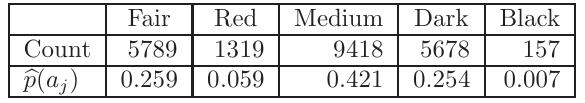
\includegraphics[width=\textwidth]{chap4-20250314.png}
% \caption{}
\label{}
\end{figure}

\begin{figure}[H]
\centering
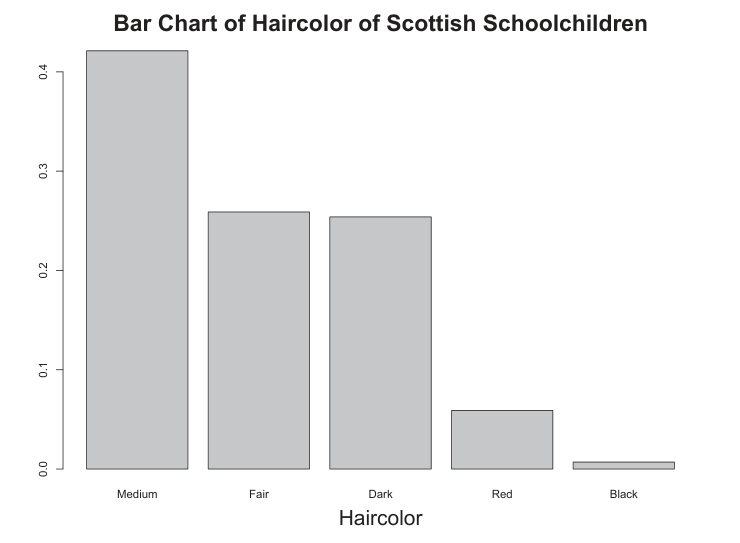
\includegraphics[width=\textwidth]{2-chap4-20250314.png}
% \caption{}
\label{}
\end{figure}

For the second case, assume that the values in the space $\mathcal{D}$ are \textbf{ordinal} in nature; i.e. the natural ordering of the $a_j$ $s$ is numerically meaningful. In this case, the usual histogram is an abutting bar chart with heights $\widehat{p}(a_j)$ that are plotted in the natural order of the $a_j$ $s$, as in the following example.

\begin{figure}[H]
\centering
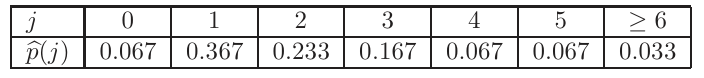
\includegraphics[width=\textwidth]{4-chap4-20250314.png}
% \caption{}
\label{}
\end{figure}

\begin{figure}[H]
\centering
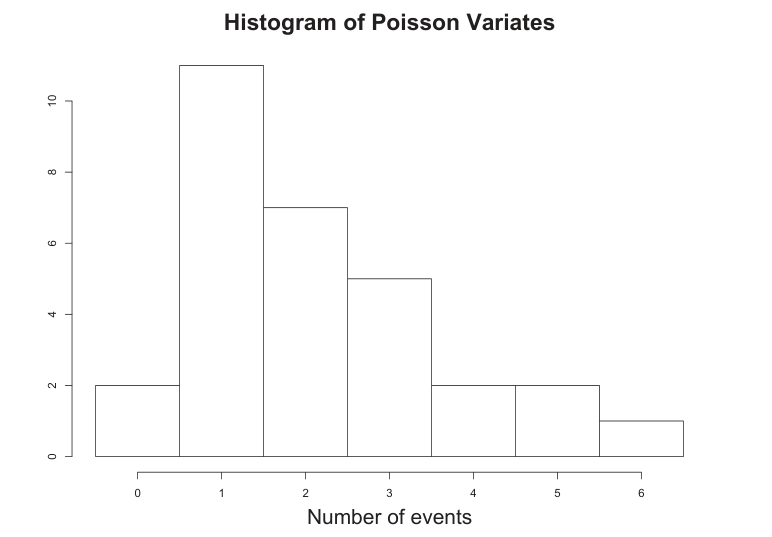
\includegraphics[width=\textwidth]{5-chap4-20250314.png}
% \caption{}
\label{}
\end{figure}

\subsubsection{Continuous Distribution}

For this section, assume that the random sample $X_1,\dots,X_n$ is from a continuous random variable $X$ with continuous pdf $f(t)$. For an arbitrary but fixed point $x$ and a given $h>0$, consider the interval $(x-h,x+h)$. By the mean value theorem for integrals, we have for some $\xi$, $\lvert x-\xi \rvert<h$, that
\[
P(x-h<X<x+h)=\int_{x-h}^{x+h} f(t) \, dt =f(\xi)2h\approx f(x)2h
\]
Let the sample items fall in $(x-h,x+h)$, which suggests the following nonparmetric extimate of $f(x)$ at a given $x$:
\[
\widehat{f}(x)=\frac{\#\{ x-h<X_i<x+h \}}{2hn}
\]
More formally, a nonparametric estimator of $f(x)$ is
\[
\widehat{f}(x)=\frac{1}{2hn}\sum_{i=1}^{n} \mathbb{1}_{(x-h,x+h)}(X_i)
\]
Then
\[
E[\widehat{f}(x)]=\frac{1}{2hn}\sum_{i=1}^{n} E[\mathbb{1}_{(x-h,x+h)}(X_i)]=\frac{1}{2hn}\sum_{i=1}^{n} P(X_i\in(x-h,x+h))=\frac{1}{2hn}nf(\xi)2h=f(\xi)\to f(x)\quad \text{as }h\to0
\]
Hence $\widehat{f}(x)$ is approximately an unbiased estimator of the density $f(x)$.

\begin{figure}[H]
\centering
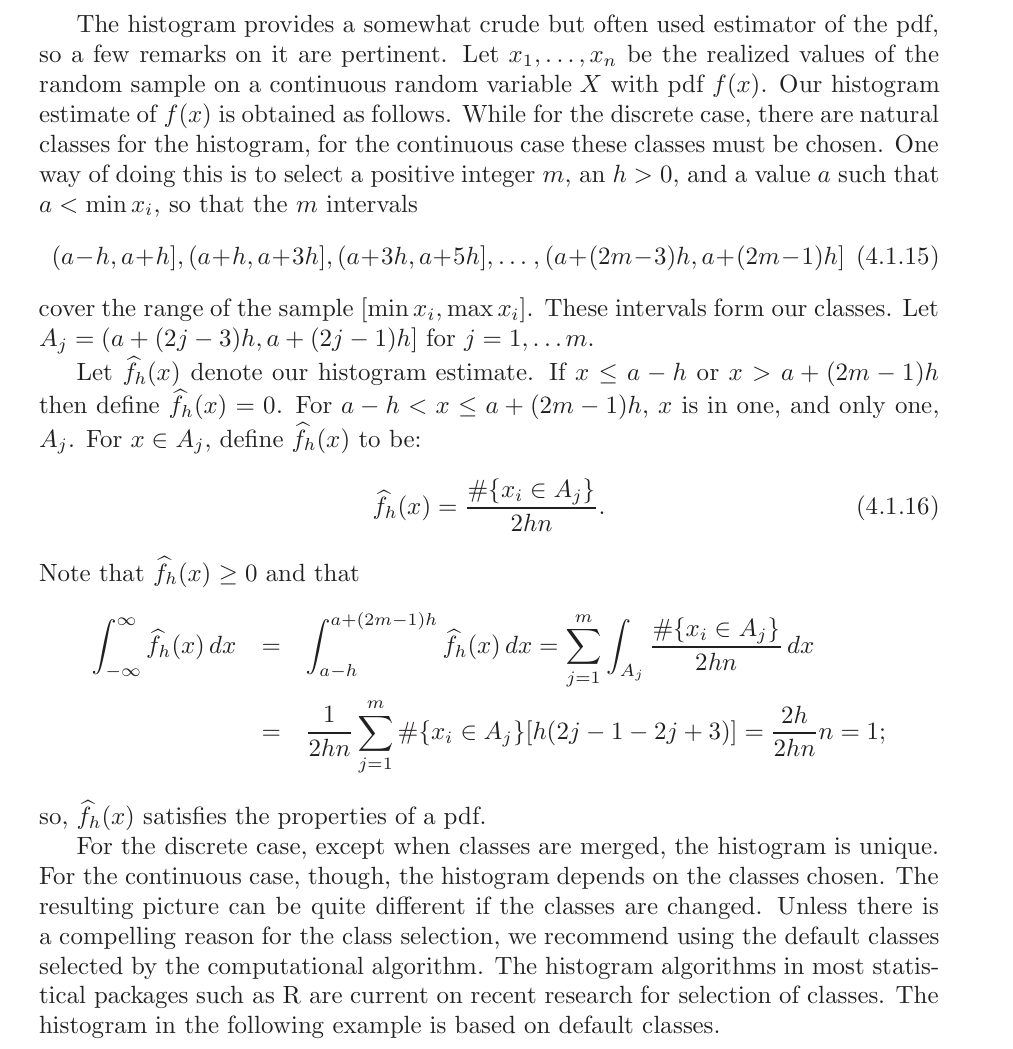
\includegraphics[width=\textwidth]{6-chap4-20250314.png}
% \caption{}
\label{}
\end{figure}

\section{Confidence Intervals}

Recall that the random variable of interest $X$ has density $f (x;\theta),\theta\in \Omega$, where $\theta$ is unknown. In Section 4.1, we discussed estimating $\theta$ by a statistic $\widehat{\theta}=\widehat{\theta}(X_1,\dots,X_n)$, where $X_1,\dots,X_n$ is a sample from the distribution of $X$. But how much did $\widehat{\theta}$ miss $\theta$? In this section, we embody this estimate of error in terms of a confidence interval, which we now formally define:

\begin{figure}[H]
\centering
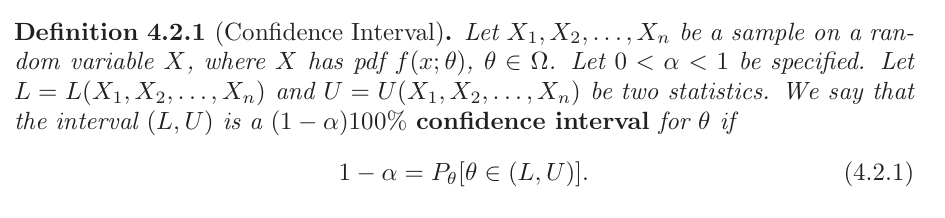
\includegraphics[width=\textwidth]{7-chap4-20250314.png}
% \caption{}
\label{}
\end{figure}

\begin{figure}[H]
\centering
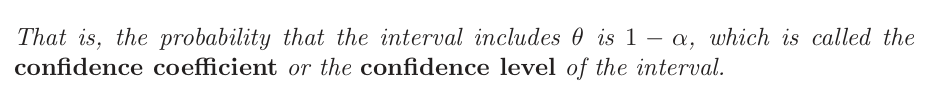
\includegraphics[width=\textwidth]{8-chap4-20250314.png}
% \caption{}
\label{}
\end{figure}

\begin{figure}[H]
\centering
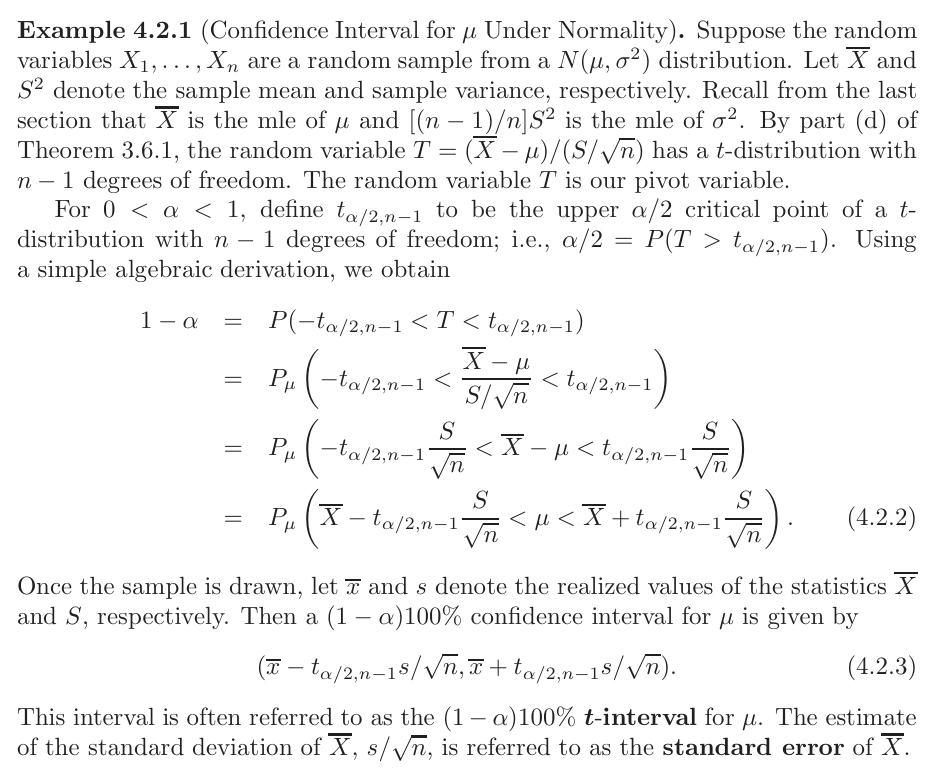
\includegraphics[width=\textwidth]{11-chap4-20250314.png}
% \caption{}
\label{}
\end{figure}

For $0<\alpha<1$, define $\alpha/2=P(Z>z_{\alpha/2 })$ for $Z\sim N(0,1)$.

Motivated by the CLT, we have
\begin{figure}[H]
\centering
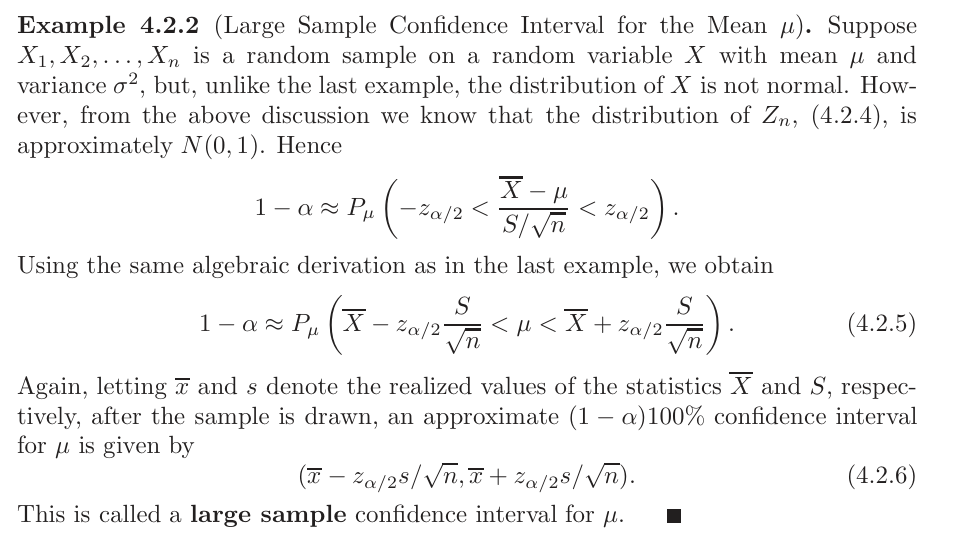
\includegraphics[width=\textwidth]{9-chap4-20250314.png}
% \caption{}
\label{}
\end{figure}

\begin{figure}[H]
\centering
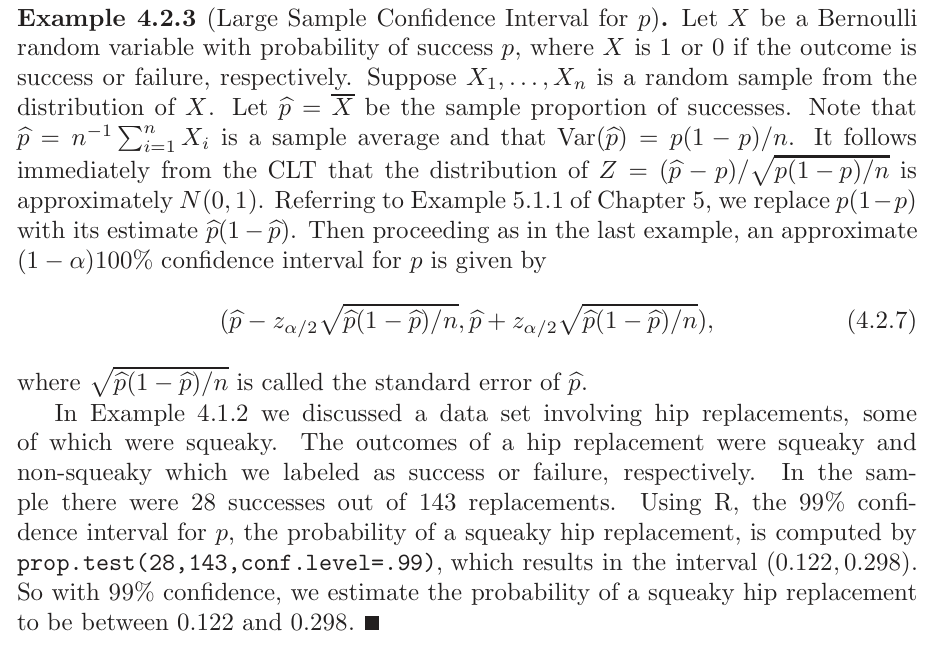
\includegraphics[width=\textwidth]{10-chap4-20250314.png}
% \caption{}
\label{}
\end{figure}

\subsection{Confidence Intervals for Difference in Means}

A practical problem of interest is the comparison of two distributions, $X$ and $Y$. In this section, we compare the means of $X$ and $Y$, denoted by $\mu_1$ and $\mu_2$. In particular, we obtain confidence intervals for the difference $\Delta=\mu_1-\mu_2$. Let $X_1,\dots,X_{n_1}$ be a random sample from the distribution of $X$ and $Y_1,\dots,Y_{n_2}$ from $Y$, and all independent of one another. Let $\overline{X}=n_1 ^{-1}\sum_{i=1}^{n_1}X_i$ and $\overline{Y}=n_2^{-1}\sum_{i=1}^{n_2}Y_i$ and $\widehat{\Delta}=\overline{X}-\overline{Y}$, which is an unbiased estimator of $\Delta$. This difference $\widehat{\Delta}-\Delta$ is the numerator of the pivot random variable. By independence of the samples,
\[
\mathrm{Var}(\widehat{\Delta})=\frac{\sigma_1^{2}}{n_1}+\frac{\sigma_2^{2}}{n_2}
\]
Let $S_1^{2}=(n_1-1)^{-1}\sum_{i=1}^{n_1}(X_i-\overline{X})^{2}$ and $S_2^{2}=(n_2-1)^{-1}\sum_{i=1}^{n_2}(Y_i-\overline{Y})^{2}$ be the sample variances. Then estimating the variances by the sample variances, consider the random variable
\[
Z=\frac{\widehat{\Delta}-\Delta}{\sqrt{ \frac{S_1^{2}}{n_1} +\frac{S_2^{2}}{n_2}}}
\]
By CLT, this pivot variable has an approximate $N(0,1)$ distribution. This leads to the approximate $(1-\alpha) 100\%$ confidence interval for $\Delta=\mu_1-\mu_2$ given by
\[
\left( (\overline{x}-\overline{y})-z_{\alpha/2}\sqrt{ \frac{s_1^{2}}{n_1}+\frac{s_2^{2}}{n_2} }, (\overline{x}-\overline{y})+z_{\alpha/2}\sqrt{ \frac{s_1^{2}}{n_1}+\frac{s_2^{2}}{n_2} }\right)
\]
where $\sqrt{ (s_1^{2}/n_1)+(s_2^{2}/n_2) }$ is the standard error of $\overline{X}-\overline{Y}$. This is a large sample $(1-\alpha) 100\%$ confidence interval for $\mu_1-\mu_2$.

\begin{figure}[H]
\centering
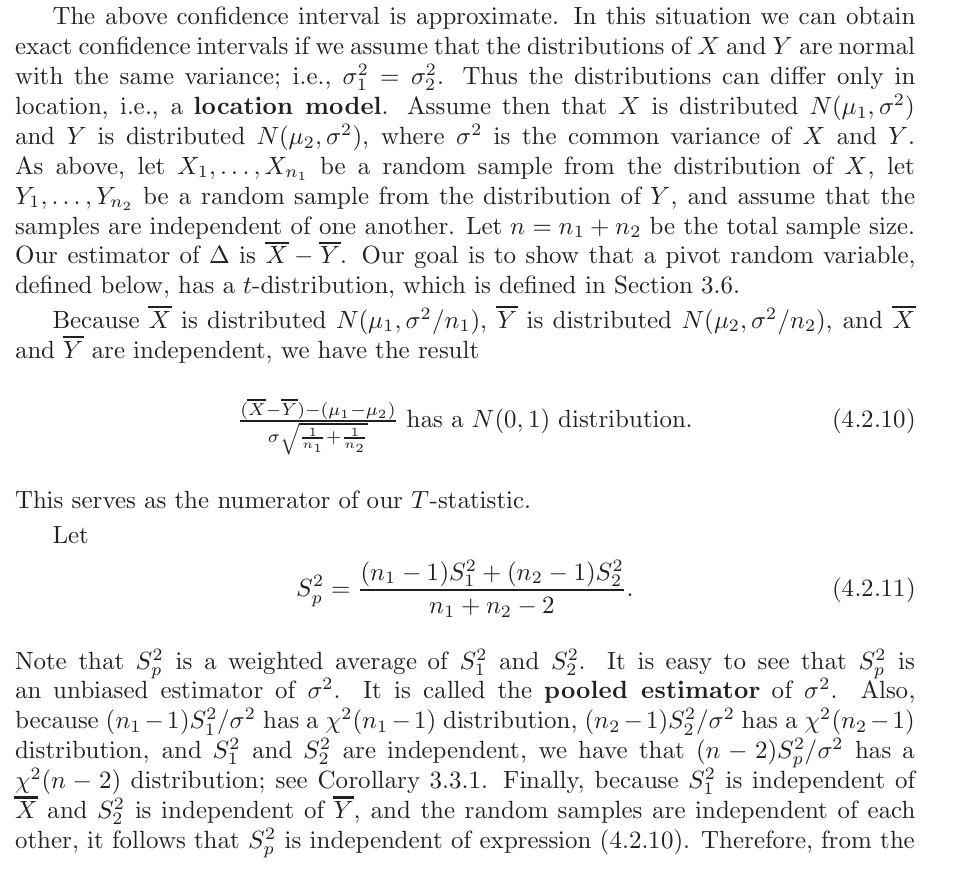
\includegraphics[width=\textwidth]{12-chap4-20250314.png}
% \caption{}
\label{}
\end{figure}

\begin{figure}[H]
\centering
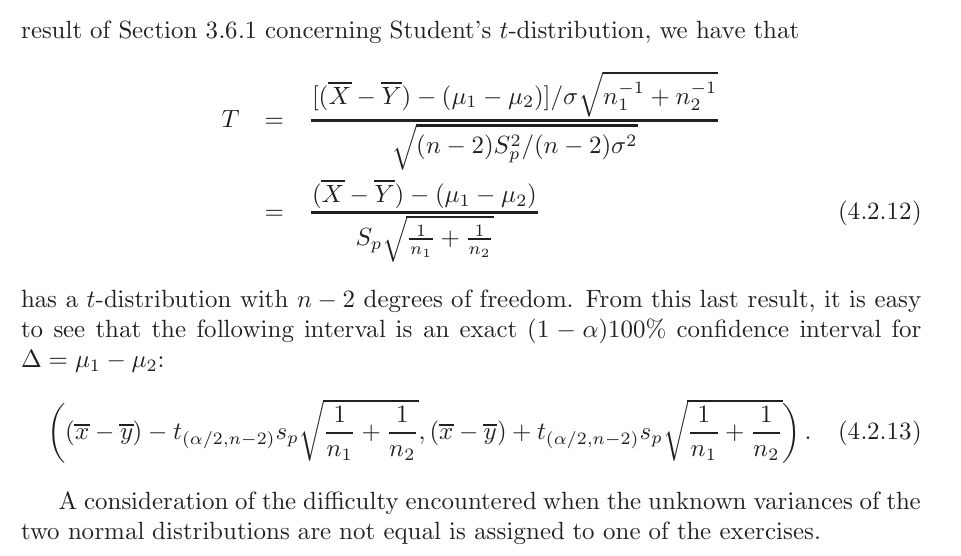
\includegraphics[width=\textwidth]{13-chap4-20250314.png}
% \caption{}
\label{}
\end{figure}

\subsection{Confidence Interval for Difference in Proportions}

Omitted...

\subsection{Confidence Intervals for Parameters of Discrete Distributions}

Omitted...

\section{Order Statistics}

\begin{definition}[order statistic]
\begin{figure}[H]
\centering
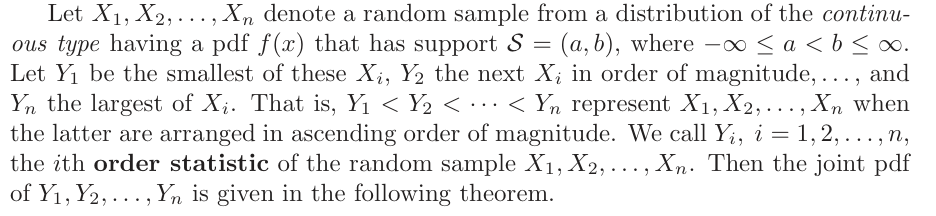
\includegraphics[width=\textwidth]{14-chap4-20250314.png}
% \caption{}
\label{}
\end{figure}
\end{definition}
\begin{figure}[H]
\centering
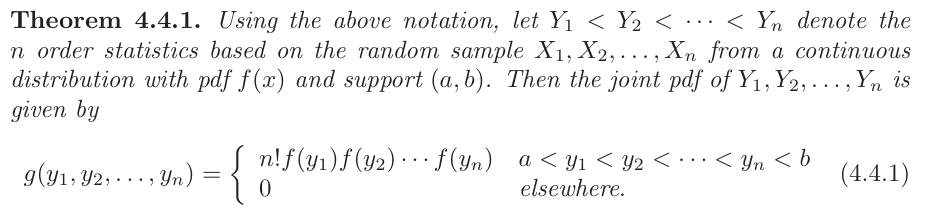
\includegraphics[width=\textwidth]{15-chap4-20250314.png}
% \caption{}
\label{}
\end{figure}

Note that the support of $X_1,\dots,X_n$ an be partitioned into $n!$ mutually disjoint sets that map onto the support of $Y_1,\dots,Y_n$ namely, $\{ (y_1,\dots,y_n):a<y_1<\dots<y_n<b \}$. One of these $n!$ sets is $a<x_1<\dots<x_n<b$, and the others can be found by permuting the $n$ $x$ s in all possible way, thus the Jacobian equal to 1.
\[
g(y_1,\dots,y_n)=\sum_{i=1}^{n!} \lvert J_i \rvert f(y_1)\dots f(y_n)=\begin{cases}
n!f(y_1)\dots f(y_n) & a<y_1<\dots<y_n<b \\
0 & \text{elsewhere}
\end{cases}
\]
\begin{figure}[H]
\centering
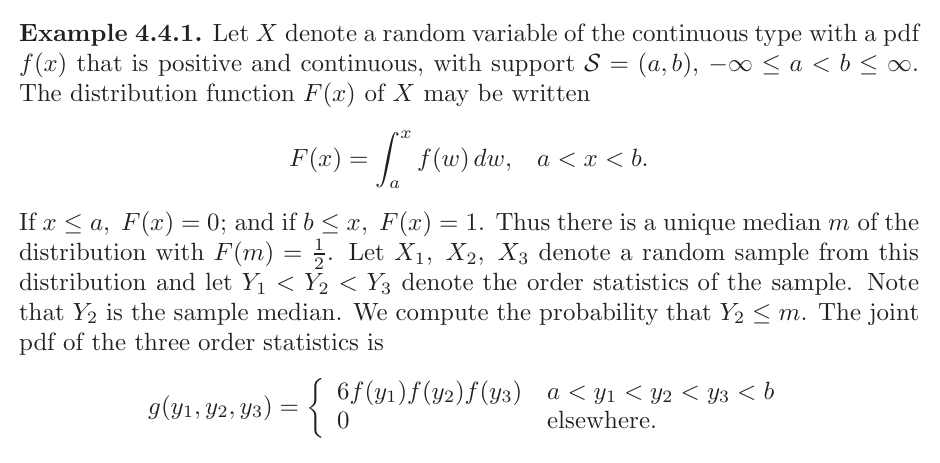
\includegraphics[width=\textwidth]{16-chap4-20250314.png}
% \caption{}
\label{}
\end{figure}

\begin{figure}[H]
\centering
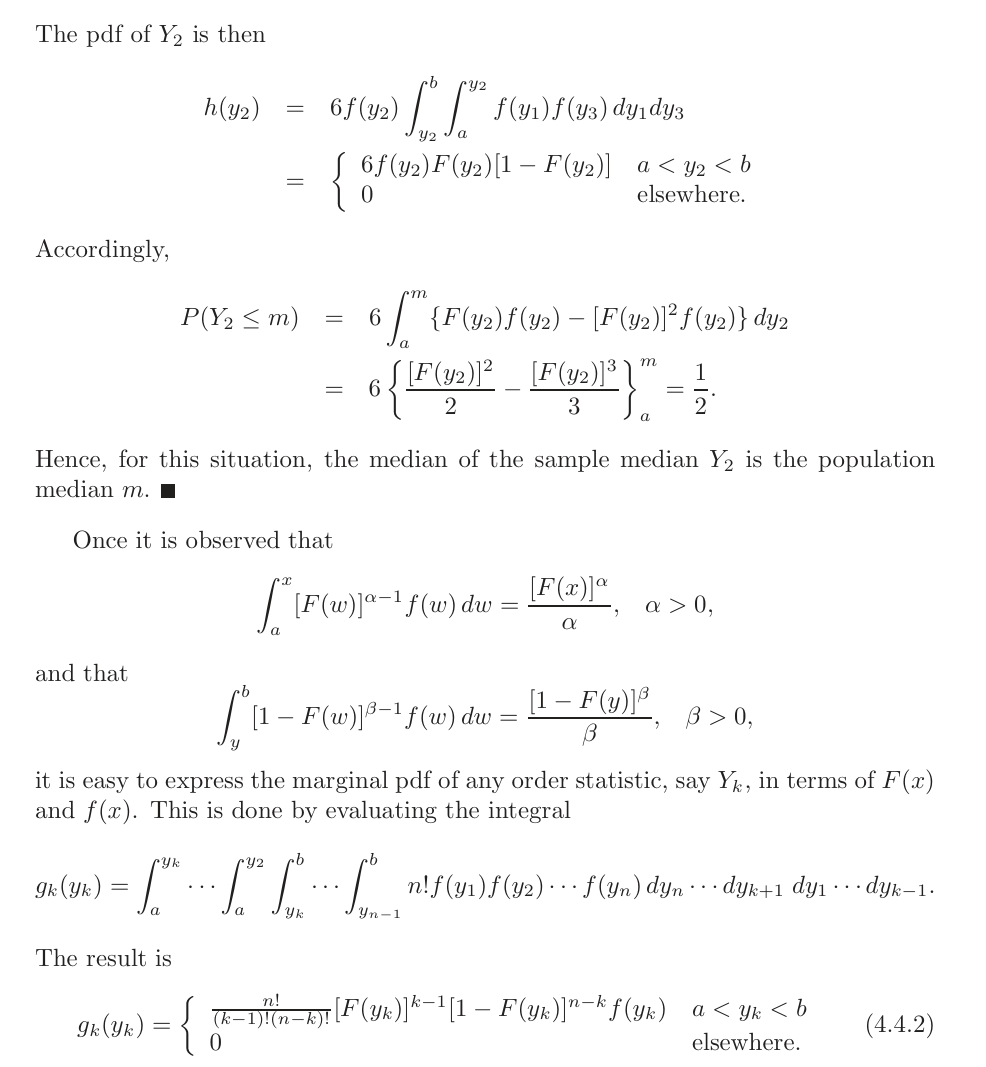
\includegraphics[width=\textwidth]{17-chap4-20250314.png}
% \caption{}
\label{}
\end{figure}

Omitted...

\subsection{Quantiles}

\subsection{Confidence Intervals for Quantiles}

$X$ continuous rv with cdf $F(x)$. For $0<p<1$, define the $100p$ th distribution percentile to be $\xi_{p}$, where $F(\xi_{p})=p$. Let $Y_1<\dots<Y_n$ be the order statistics. Then
\[
P(Y_i<\xi_{p}<Y_j)=\sum_{w=i}^{j-1} \binom{n}{w}p^{w}(1-p)^{n-w}\eqqcolon \gamma
\]
Then $(y_i,y_j)$ serves as a $100\gamma\%$ confidence interval for $\xi_{p}$, the quantile of order $p$.

\subsubsection{Confidence Interval for the Median}

\begin{figure}[H]
\centering
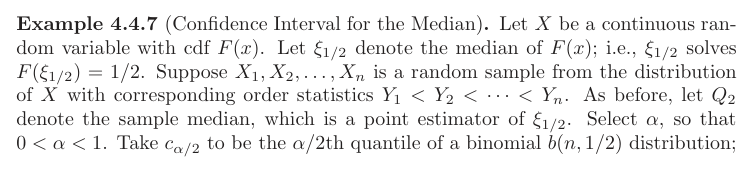
\includegraphics[width=\textwidth]{chap4-2025033022.png}
% \caption{}
\label{}
\end{figure}
\begin{figure}[H]
\centering
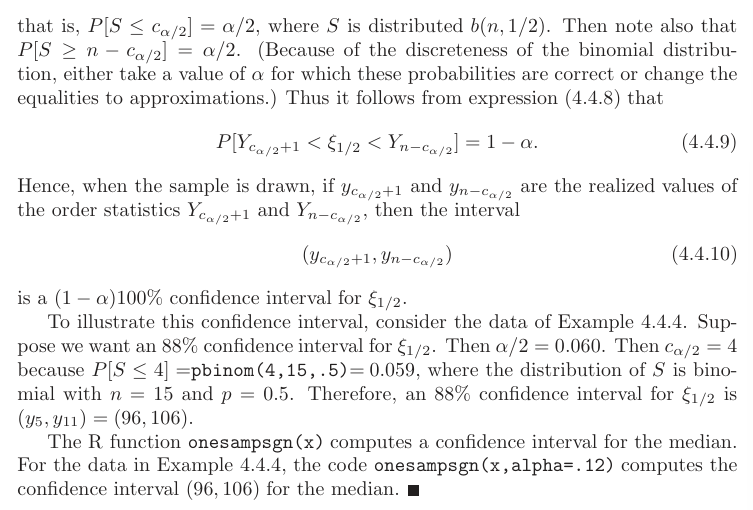
\includegraphics[width=\textwidth]{1-chap4-2025033022.png}
% \caption{}
\label{}
\end{figure}

\section{Introduction to Hypothesis Testing}

See All of statistics Chapter 10.

\subsection{Definitions of critical (rejection) region, power function, size (significance level), level, type I (II) error, two-side test, one-side test}

We partition the parameter space $\Theta$ into two disjoint sets $\Theta_0$ and $\Theta_1$ and we wish to test
\[
H_0:\theta\in\Theta_0\qquad \text{versus}\qquad H_1:\theta\in\Theta_1
\]
We call $H_0$ the \textbf{null hypothesis} and $H_1$ the \textbf{alternative hypothesis}. Let $X$ be a r.v. and $\mathcal{X}$ be the range of $X$. To test a hypothesis, we aim to find the \textbf{rejection region}(critical region) $R\subset \mathcal{X}$. If $X\in R$ we reject $H_0$, otherwise retain $H_0$.

\begin{definition}[critical region (rejection region)]
A test of $H_0$ versus $H_1$ is based on a subset $C$ of $\mathcal{D}$. This set $C$ is called the \textbf{critical region (rejection region)} and its corresponding decision rule (test) is
\[
\begin{aligned} \text { Reject } H_0\left(\text { Accept } H_1\right) &\qquad  \text { if }\left(X_1, \ldots, X_n\right) \in C \\ \text { Retain } H_0\left(\text { Reject } H_1\right) & \qquad \text { if }\left(X_1, \ldots, X_n\right) \in C^c .\end{aligned}
\]
\end{definition}
Usually, the \textbf{rejection region} $R$ (critical region $C$) is of the form
\[
R=\{ x:T(x)>c \}
\]
where $T$ is a \textbf{test statistic} and $c$ is called a \textbf{critical value}.

\begin{definition}[power function, size (significance level), level]
The \textbf{power function} of a test with rejection region $R$ is defined by
\[
\beta(\theta)=\mathbb{P}_{\theta}(X\in R)
\]
The \textbf{size} of a test is defined to be
\[
\alpha=\sup_{\theta\in\Theta_0}\beta(\theta)
\]
A test is said to have \textbf{level}\footnote{The definition is useless.} $\alpha$ if its size is less than or equal to $\alpha$.
\end{definition}
\begin{definition}[type I error, type II error]
Rejecting $H_0$ when $H_0$ is true is called a \textbf{type I error}. Retaining $H_0$ when $H_1$ is true is called a \textbf{type II error}.
\end{definition}
\begin{definition}[two-side test, one-side test]
A test of the form
\[
H_0:\theta=\theta_0\qquad \text{versus}\qquad H_1:\theta\neq \theta_0
\]
is called a \textbf{two-side test}. A test of the form
\[
H_0:\underset{ \text{or }\geq  }{ \theta\leq \theta_0 }\qquad \text{versus}\qquad H_1:\underset{ \text{or }< }{ \theta>\theta_0 }
\]
is called a \textbf{one-side test}. The most common tests are two-sided.
\end{definition}
\subsubsection{Example}

\begin{figure}[H]
\centering
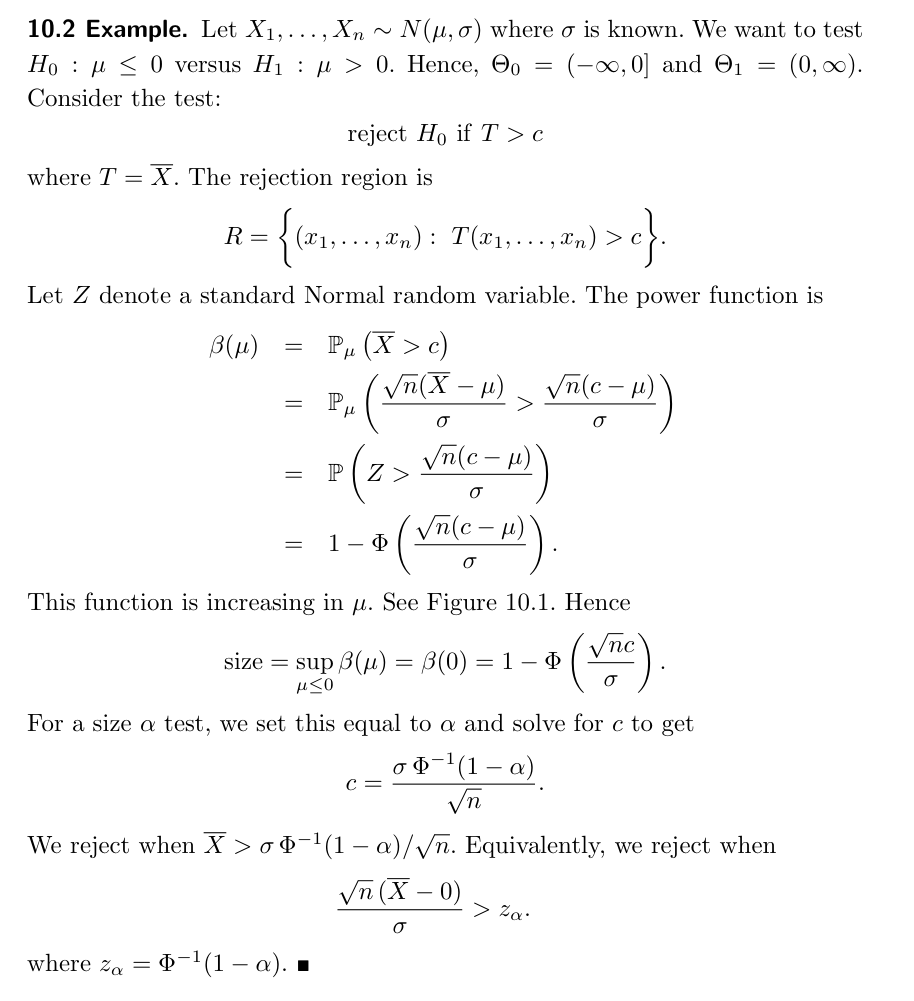
\includegraphics[width=\textwidth]{4-chap4-2025040315.png}
% \caption{}
\label{}
\end{figure}

\begin{figure}[H]
\centering
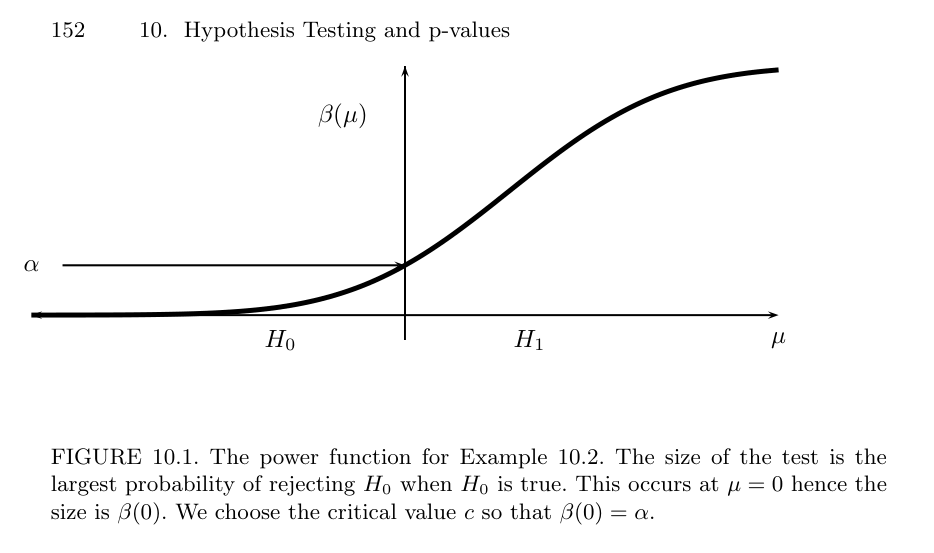
\includegraphics[width=\textwidth]{5-chap4-2025040315.png}
% \caption{}
\label{}
\end{figure}

Next we consider four widely used tests: the Wald test, the $\chi^{2}$ test, the permutation test, and the likelihood ratio test.

\subsection{The Wald test}

Let $\theta$ be a scalar parameter, let $\widehat{\theta}$ be an estimate of $\theta$ and let $\widehat{\text{se}}$ be the estimated standard error of $\widehat{\theta}$.

\begin{definition}[The Wald Test]
Consider testing $H_0:\theta=\theta_0,H_1:\theta\neq\theta_0$. Assume that the estimator $\widehat{\theta}$ is asymptotically Normal, i.e.
\[
W\coloneqq \frac{\widehat{\theta}-\theta_0}{\widehat{\text{se}}}\overset{ \mathcal{D} }{ \to }N(0,1)
\]
The size $\alpha$ \textbf{Wald test} is: reject $H_0$ when $\lvert W \rvert>z_{\alpha/2}$.
\end{definition}
$z_{\alpha}$ means that for $Z\sim N(0,1)$,
\[
\mathbb{P}(Z>z_{\alpha})=\alpha
\]
Thus
\[
z_{\alpha}\coloneqq \Phi ^{-1}(1-\alpha)
\]
where $\Phi(x)=\mathbb{P}(Z\leq x)=F_{Z}(x)$.

\begin{remark}
An alternative version of the Wald test statistic is $W=(\widehat{\theta}-\theta_0)/\widehat{\text{se}_{0}}$ where $\text{se}_{0}$ is the standard error computed at $\theta=\theta_0$. Both versions of the test is valid.
\end{remark}
Let us consider the power of the Wald test when the null hypothesis is false.
\begin{figure}[H]
\centering
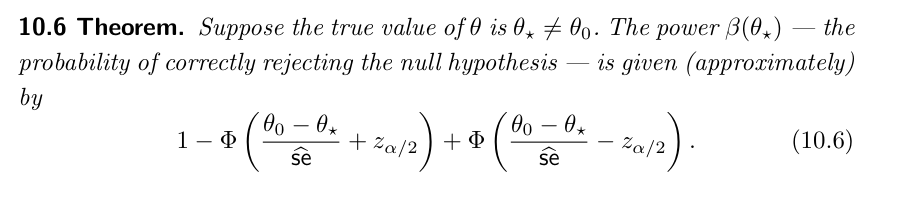
\includegraphics[width=\textwidth]{9-chap4-2025040315.png}
% \caption{}
\label{}
\end{figure}

\begin{theorem}[The rejection region of size $\alpha$ Wald test]
The size $\alpha$ Wald test rejects $H_0:\theta=\theta_0$ versus $H_1:\theta\neq\theta_0$ iff $\theta_0 \not\in C$ where
\[
C=(\widehat{\theta}-\widehat{\text{se}}\cdot z_{\alpha/2},\widehat{\theta}+\widehat{\text{se}}\cdot z_{\alpha/2})
\]
Thus, testing the typothesis is equivalent to checking whether the null value is in the confidence interval.
\end{theorem}
\begin{remark}
When we reject $H_0$ we often say that the result is statistically significant.
\end{remark}
\subsubsection{Example 1}

\begin{figure}[H]
\centering
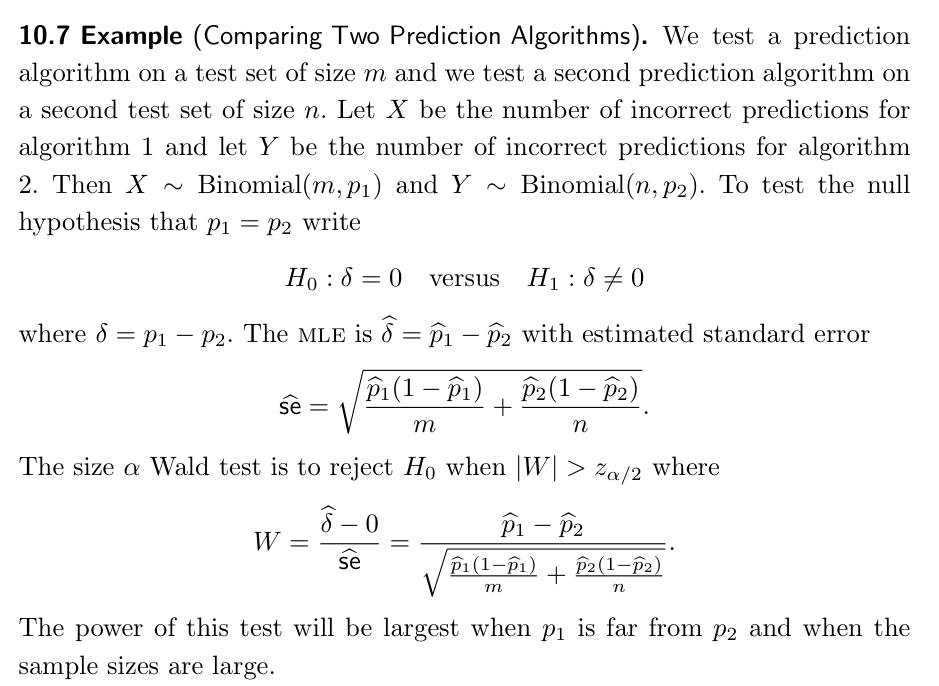
\includegraphics[width=\textwidth]{5-chap4-2025041621.png}
% \caption{}
\label{}
\end{figure}

\subsubsection{Example 2}

\begin{figure}[H]
\centering
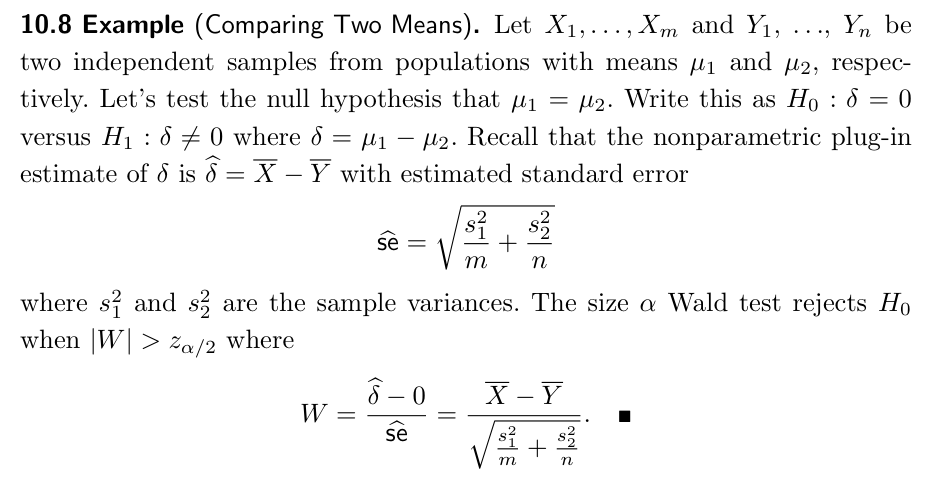
\includegraphics[width=\textwidth]{6-chap4-2025041621.png}
% \caption{}
\label{}
\end{figure}

\subsection{\texorpdfstring{$p$}{p} -values}

For every $\alpha\in(0,1)$ we have a size $a$ test with rejection region $R_{\alpha}$. Then
\[
\text{p-value}=\inf \{ \alpha:T(X)\in R_{\alpha} \}
\]
$p$ -value is the smallest level at which we can reject $H_0$.

\begin{remark}
Do not confuse the $p$ -value with $\mathbb{P}(H_0|\text{Data})$. The $p$ -value is not the probability that the null hypothesis is true.
\end{remark}
Suppose that the size $\alpha$ test is of the form
\[
\text{reject  }H_0\qquad \text{iff}\qquad T(X)\geq c_{\alpha}
\]
Then
\[
\text{p-value}=\sup_{\theta\in\Theta_0}\mathbb{P}_{\theta}(T(X)>T(x))
\]
where $x$ is the observed value of $X$.

\begin{note}
The $p$ -value is the probability (under $H_0$) of observing a value of the test statistic the same as or more extreme than what was actually observed.
\end{note}
\subsubsection{Example}

\begin{figure}[H]
\centering
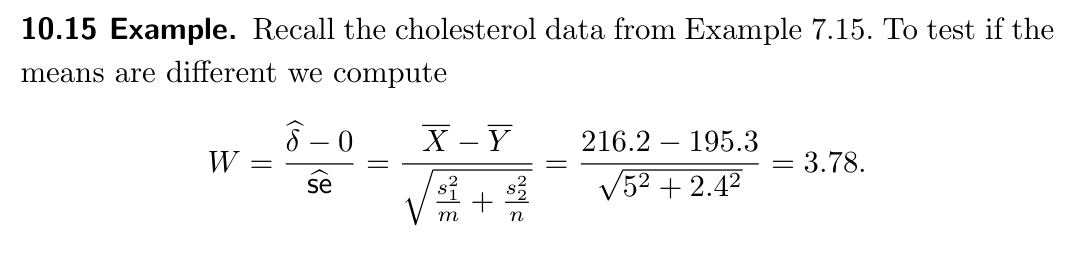
\includegraphics[width=\textwidth]{3-chap4-2025040316.png}
% \caption{}
\label{}
\end{figure}
\begin{figure}[H]
\centering
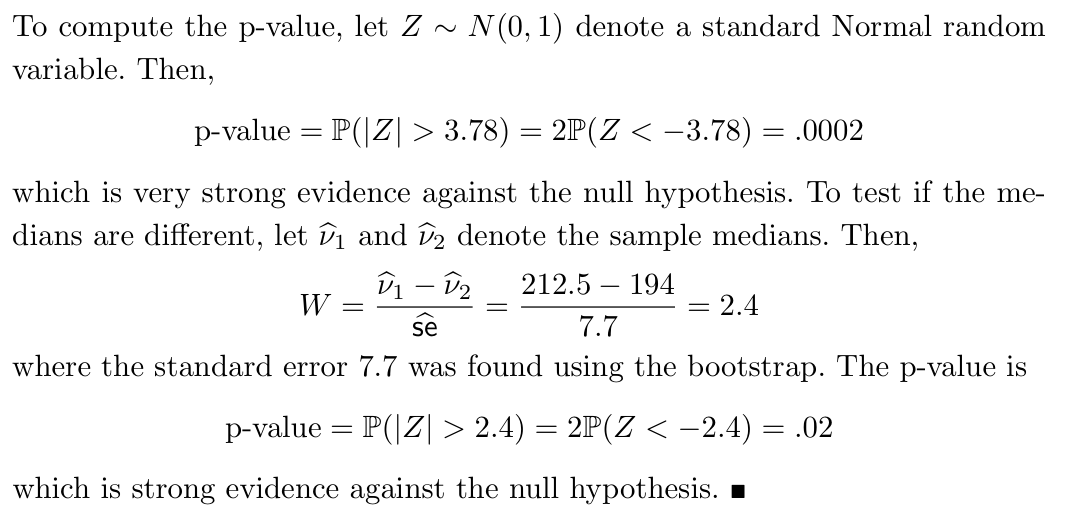
\includegraphics[width=\textwidth]{4-chap4-2025040316.png}
% \caption{}
\label{}
\end{figure}

\subsection{\texorpdfstring{$\chi^{2}$}{chi^2} test}

\subsubsection{Definition of \texorpdfstring{$\chi^{2}$}{chi^2} distribution}

\begin{figure}[H]
\centering
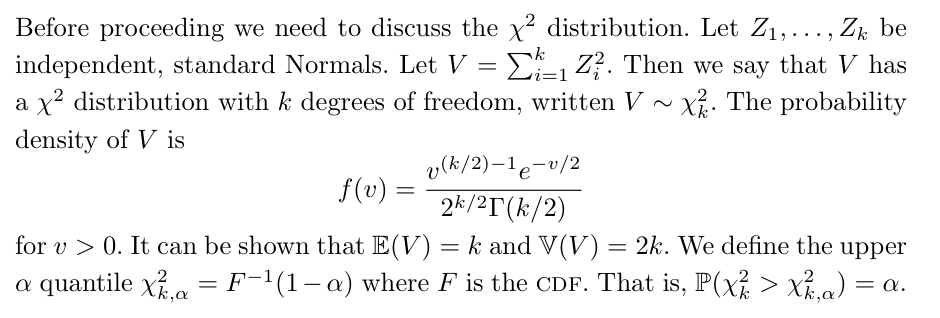
\includegraphics[width=\textwidth]{chap4-2025041621.png}
% \caption{}
\label{}
\end{figure}

\subsubsection{Pearson's \texorpdfstring{$\chi^{2}$}{chi^2} test for multinomial data}

The Pearson's $\chi^{2}$ test is used for multinomial data. If $X=(X_1,\dots,X_k)$ has a multinomial $(n,p)$ distribution, then the MLE of $p$ is $\widehat{p}=(\widehat{p}_{1},\dots,\widehat{p}_k)$

\begin{note}
$X_1,\dots,X_k$ need not to be independent!
\end{note}
\begin{definition}[Pearson's $\chi^{2}$ statistic]
\textbf{Pearson's $\chi^{2}$ statistic} is
\[
T=\sum_{j=1}^{k} \frac{(X_j-np_{0j})^2}{np_{0j}}=\sum_{j=1}^{k}\frac{(X_j-E_j)^2}{E_j} 
\]
where $E_j=\mathbb{E}(X_j)=np_{0j}$ is the expected value of $X_j$ under $H_0$.
\end{definition}
Under $H_0$, $T \rightsquigarrow \chi_{k-1}^2$. Hence the test: reject $H_0$ if $T>$ $\chi_{k-1, \alpha}^2$ has asymptotic level $\alpha$. The p-value is $\mathbb{P}\left(\chi_{k-1}^2>t\right)$ where $t$ is the observed value of the test statistic.

\begin{figure}[H]
\centering
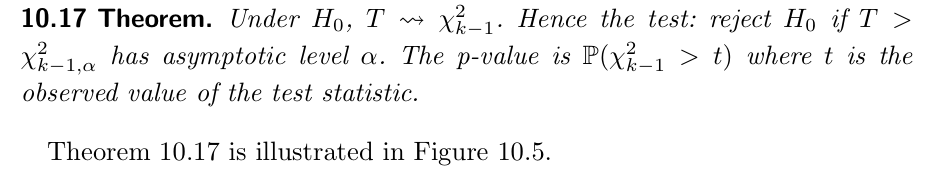
\includegraphics[width=\textwidth]{2-chap4-2025041621.png}
% \caption{}
\label{}
\end{figure}

\paragraph{Example}

\begin{figure}[H]
\centering
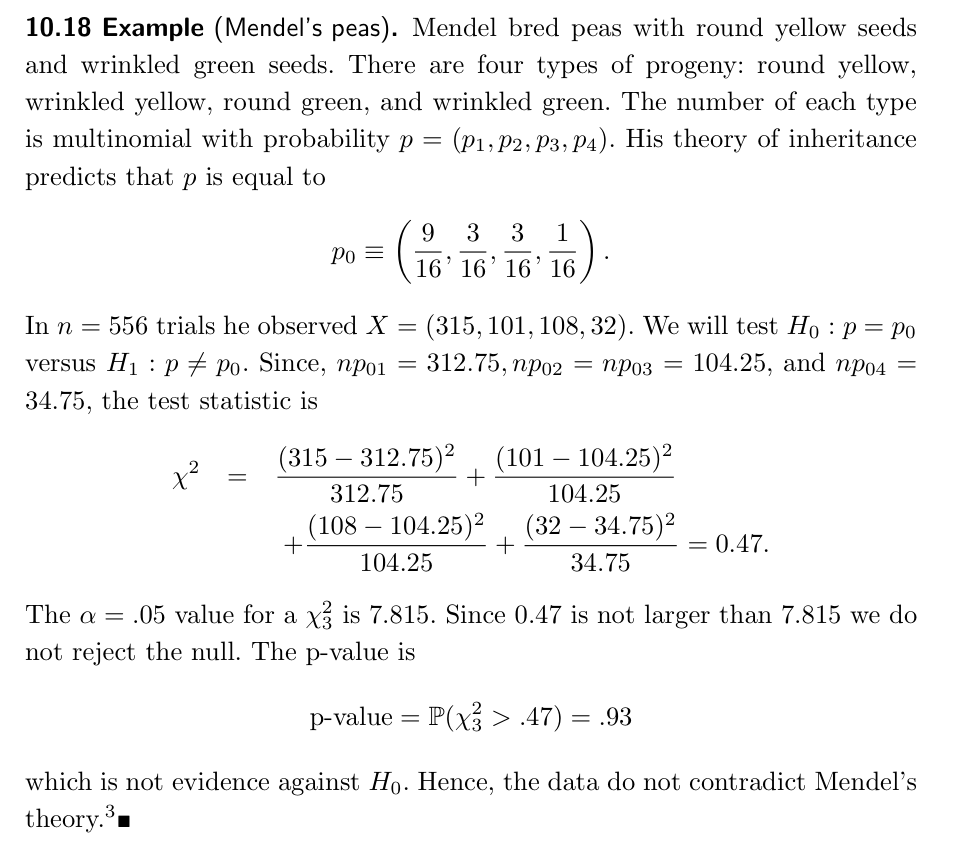
\includegraphics[width=\textwidth]{4-chap4-2025041621.png}
% \caption{}
\label{}
\end{figure}

\subsubsection{Goodness-of-fit test (\texorpdfstring{$H_0:$}{H_0:} \texorpdfstring{$Y$}{Y} satisfies some distribution)}

\begin{figure}[H]
\centering
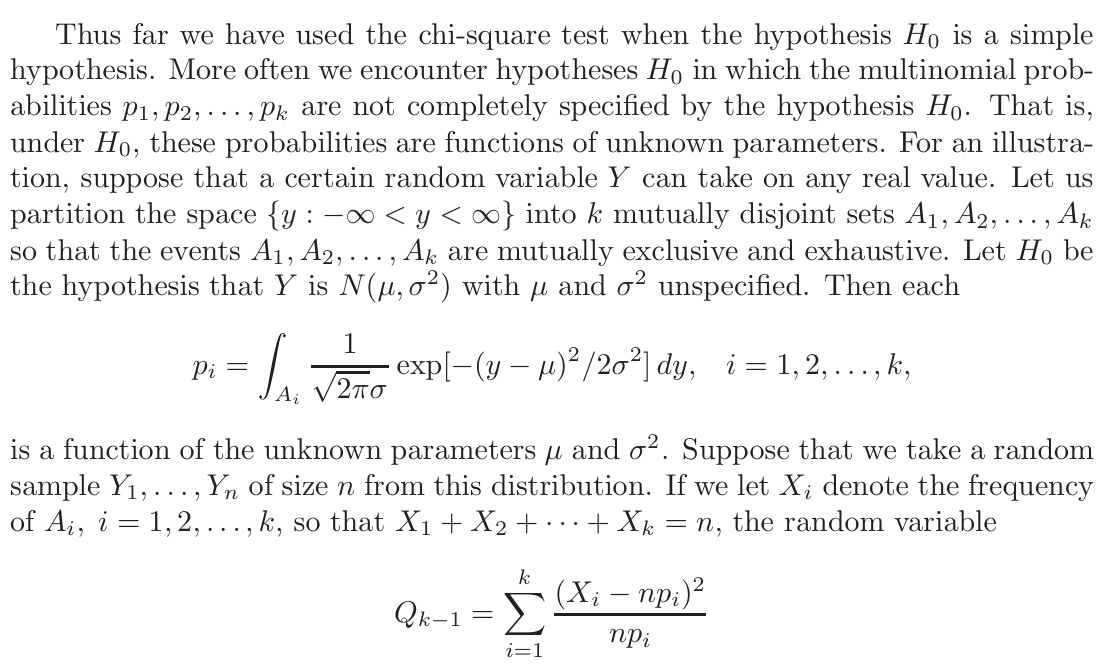
\includegraphics[width=\textwidth]{1-chap4-2025041712.png}
% \caption{}
\label{}
\end{figure}
\begin{figure}[H]
\centering
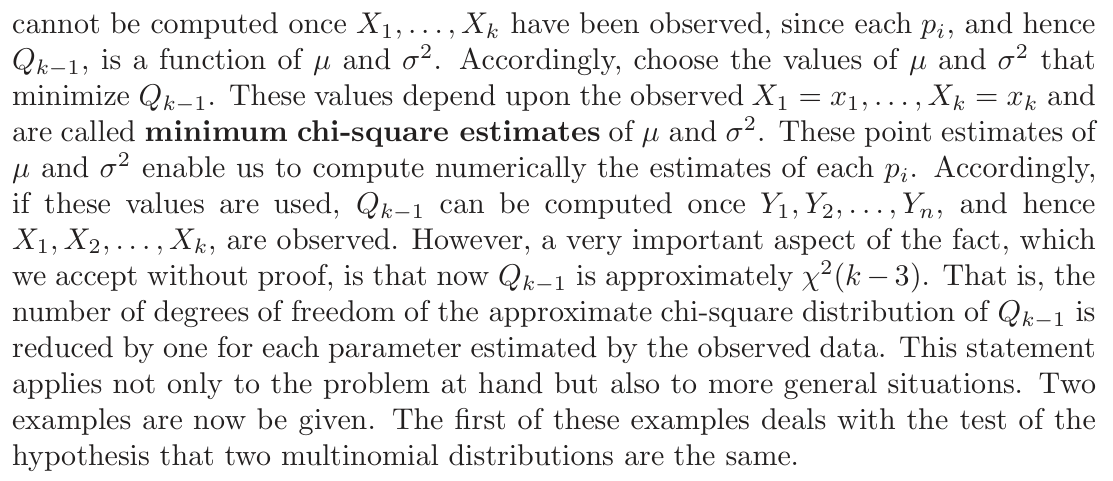
\includegraphics[width=\textwidth]{2-chap4-2025041712.png}
% \caption{}
\label{}
\end{figure}
